\documentclass[10pt,letterpaper]{article}
\usepackage[margin=0.75in,top=0.75in,bottom=0.75in]{geometry}
\usepackage{amsmath,amssymb}
\usepackage{fontspec}
\setmainfont{Inter}[
    UprightFont = *-Regular,
    BoldFont = *-Bold,
    ItalicFont = *-Regular,
    BoldItalicFont = *-Bold
]
\setmonofont{Liberation Mono}[Scale=0.85]
\usepackage{graphicx}
\usepackage[dvipsnames]{xcolor}
\usepackage{fancyhdr}
\usepackage{listings}
\usepackage{tabularx}
\usepackage{booktabs}
\usepackage{longtable}
\usepackage{float}
\usepackage[colorlinks=true,linkcolor=MidnightBlue,urlcolor=MidnightBlue,citecolor=MidnightBlue,linktoc=all]{hyperref}

% Light Theme Colors (matching HW1/HW2/HW3)
\definecolor{answerblue}{RGB}{0, 70, 204}
\definecolor{headergray}{RGB}{80, 80, 80}
\definecolor{linegray}{RGB}{200, 200, 200}
\definecolor{titlecolor}{RGB}{17, 17, 17}
\definecolor{bodycolor}{RGB}{25, 25, 25}
\definecolor{codebg}{RGB}{246, 248, 252}
\definecolor{codeborder}{RGB}{208, 218, 232}

% Section styling commands matching course standard
\newcommand{\mysection}[1]{%
    \vspace{6pt}%
    {\large\bfseries\color{titlecolor} #1}\par
    \vspace{-4pt}\rule{\textwidth}{0.6pt}\vspace{4pt}%
}
\newcommand{\mysubsection}[1]{%
    \vspace{4pt}%
    {\normalsize\bfseries\color{titlecolor} #1}\par\vspace{2pt}%
}
\newcommand{\mysubsubsection}[1]{%
    \vspace{3pt}%
    {\small\bfseries\color{titlecolor} #1}\par\vspace{1pt}%
}

\lstset{
    basicstyle=\ttfamily\scriptsize\color{bodycolor},
    backgroundcolor=\color{codebg},
    frame=single,
    rulecolor=\color{codeborder},
    breaklines=true,
    showstringspaces=false,
    tabsize=2,
    xleftmargin=6pt,
    xrightmargin=6pt,
    framesep=4pt
}

\pagestyle{fancy}
\fancyhf{}
\setlength{\headheight}{20pt}
\addtolength{\topmargin}{-8pt}
\fancyhead[L]{\small\textbf{CS/DSAI-4513 Database Management Systems}}
\fancyhead[R]{\small Khor, Arika \quad$|$\quad ID: 113540292 \quad$|$\quad Report}
\fancyfoot[C]{\small\thepage}
\renewcommand{\headrulewidth}{0.4pt}
\renewcommand{\footrulewidth}{0pt}
\setlength{\parindent}{0pt}
\setlength{\parskip}{2.5pt}

\begin{document}
\color{bodycolor}

\begin{titlepage}
\centering
\vspace*{1.5cm}
{\Large\textbf{THE UNIVERSITY OF OKLAHOMA}}\\[0.3cm]
{\large School of Computer Science \& Data Science and AI}\\[2.0cm]
{\Huge\textbf{\color{answerblue}A JOB-SHOP ACCOUNTING SYSTEM}}\\[0.5cm]
{\Large\textbf{End-to-End Conceptual, Relational \& Cloud DBMS Implementation}}\\[2.5cm]
\begin{tabular}{ll}
\textbf{Course Name \& Number:} & CS/DSAI-4513 Database Management Systems \\
\textbf{Section Number:}        & Section 001 \\
\textbf{Semester \& Year:}       & Fall 2026 \\
\textbf{Instructor:}            & Dr. Le Gruenwald \\
\textbf{Author / Student Name:} & Arika Khor \\
\textbf{Student ID:}             & 113540292 \\
\textbf{Student Email:}          & Arika.S.Khor-1@ou.edu \\
\textbf{Due Date:}               & November 10, 2026 (5:00 PM CST) \\
\end{tabular}
\vfill
{\small Project Report \quad$|$\quad Microsoft Azure SQL Cloud Database}\\[0.5cm]
\end{titlepage}

\newpage
\pdfbookmark[1]{SECTION IV. TABLE OF CONTENTS}{sec:toc}
\mysection{SECTION IV. TABLE OF CONTENTS}
\vspace{0.2cm}
\renewcommand{\contentsname}{\vspace{-24pt}}
{\small
\tableofcontents
}

\newpage
\phantomsection\label{sec:task1}\addcontentsline{toc}{section}{Task 1. Entity-Relationship (ER) Diagram}
\mysection{Task 1. Entity-Relationship (ER) Diagram}
\noindent The ER diagram models the Job-Shop Accounting System in Silberschatz Chen notation. Rectangles represent entities, diamonds denote relationships, triangles represent ISA specializations, and ovals contain attributes with primary keys underlined.
\\[0.2cm]
Process, Job, and Account hierarchies use disjoint (d) partial specialization. The Job entity directly links an Assembly and a Process, and Cost Transactions update corresponding accounts when recorded.
\vspace{0.4cm}
\begin{figure}[H]
\centering
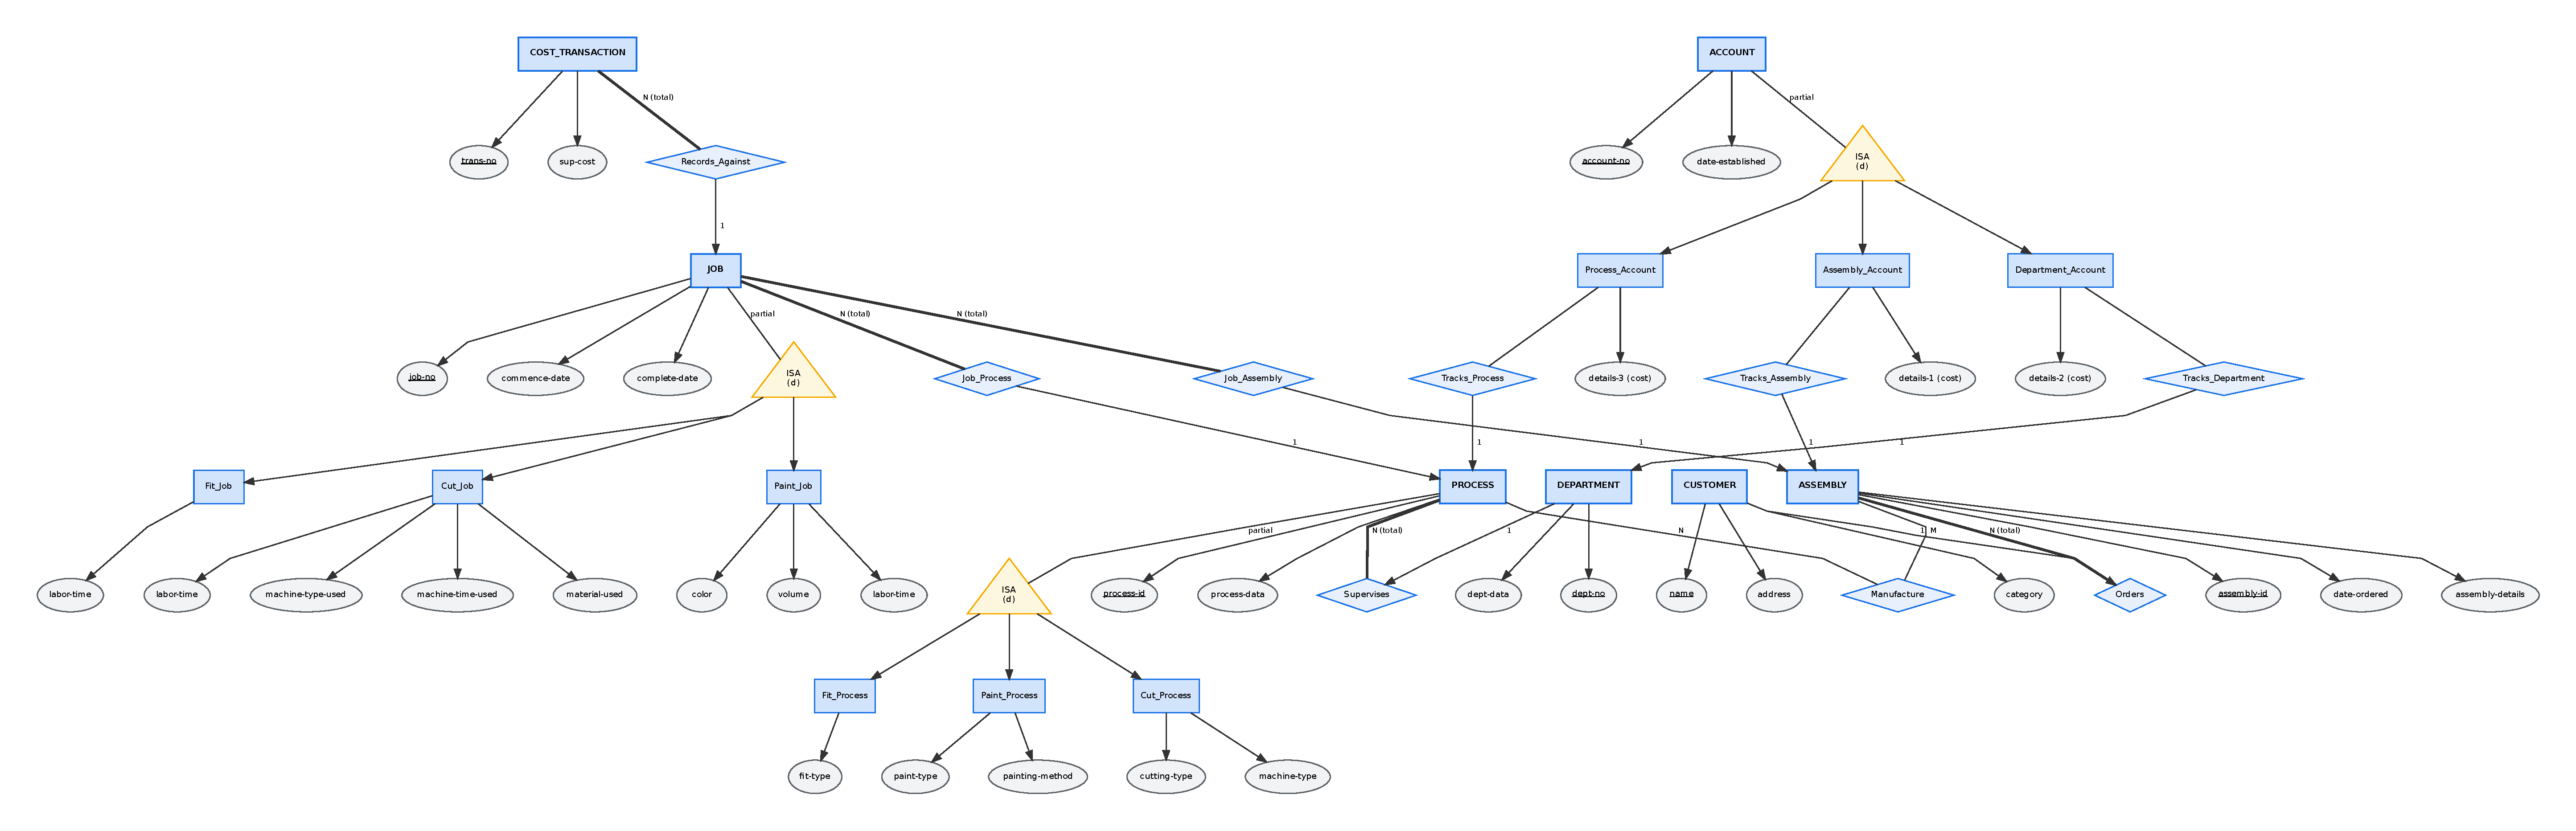
\includegraphics[width=0.98\textwidth]{../er_diagram/job_shop_er.pdf}
\caption{Silberschatz ER Diagram for Job-Shop Accounting System.}
\end{figure}

\newpage
\phantomsection\label{sec:task2}\addcontentsline{toc}{section}{Task 2. Relational Database Schemas}
\mysection{Task 2. Relational Database Schemas}
\noindent Relational schemas converted from the ER diagram using standard reduction rules. Underlined attributes form primary keys and asterisks denote foreign keys.
\\[0.3cm]
\mysubsection{1. Formal Relational Schemas}
\begin{table}[H]
\centering\scriptsize
\renewcommand{\arraystretch}{1.1}
\begin{tabularx}{\textwidth}{p{2.5cm}Xp{4.4cm}}
\toprule
\textbf{Table Name} & \textbf{Relational Schema} & \textbf{Foreign Key References} \\
\midrule
Customer & \texttt{Customer(\underline{name}, address, category)} & None \\
Assembly & \texttt{Assembly(\underline{assembly\_id}, date\_ordered, assembly\_details, customer\_name)} & \texttt{customer\_name} $\to$ \texttt{Customer.name} \\
Department & \texttt{Department(\underline{dept\_no}, dept\_data)} & None \\
Process & \texttt{Process(\underline{process\_id}, process\_data, dept\_no)} & \texttt{dept\_no} $\to$ \texttt{Department.dept\_no} \\
Fit\_Process & \texttt{Fit\_Process(\underline{process\_id}, fit\_type)} & \texttt{process\_id} $\to$ \texttt{Process.process\_id} \\
Paint\_Process & \texttt{Paint\_Process(\underline{process\_id}, paint\_type, painting\_method)} & \texttt{process\_id} $\to$ \texttt{Process.process\_id} \\
Cut\_Process & \texttt{Cut\_Process(\underline{process\_id}, cutting\_type, machine\_type)} & \texttt{process\_id} $\to$ \texttt{Process.process\_id} \\
Manufacture & \texttt{Manufacture(\underline{assembly\_id}, \underline{process\_id})} & \texttt{assembly\_id} $\to$ \texttt{Assembly}, \texttt{process\_id} $\to$ \texttt{Process} \\
Job & \texttt{Job(\underline{job\_no}, assembly\_id, process\_id, commence\_date, complete\_date)} & \texttt{assembly\_id} $\to$ \texttt{Assembly}, \texttt{process\_id} $\to$ \texttt{Process} \\
Cut\_Job & \texttt{Cut\_Job(\underline{job\_no}, machine\_used, time\_used, material, labor\_time)} & \texttt{job\_no} $\to$ \texttt{Job.job\_no} \\
Paint\_Job & \texttt{Paint\_Job(\underline{job\_no}, color, volume, labor\_time)} & \texttt{job\_no} $\to$ \texttt{Job.job\_no} \\
Fit\_Job & \texttt{Fit\_Job(\underline{job\_no}, labor\_time)} & \texttt{job\_no} $\to$ \texttt{Job.job\_no} \\
Account & \texttt{Account(\underline{account\_no}, date\_established)} & None \\
Assembly\_Account & \texttt{Assembly\_Account(\underline{account\_no}, assembly\_id, details\_1)} & \texttt{account\_no} $\to$ \texttt{Account}, \texttt{assembly\_id} $\to$ \texttt{Assembly} \\
Department\_Account & \texttt{Department\_Account(\underline{account\_no}, dept\_no, details\_2)} & \texttt{account\_no} $\to$ \texttt{Account}, \texttt{dept\_no} $\to$ \texttt{Department} \\
Process\_Account & \texttt{Process\_Account(\underline{account\_no}, process\_id, details\_3)} & \texttt{account\_no} $\to$ \texttt{Account}, \texttt{process\_id} $\to$ \texttt{Process} \\
Cost\_Transaction & \texttt{Cost\_Transaction(\underline{trans\_no}, job\_no, sup\_cost)} & \texttt{job\_no} $\to$ \texttt{Job.job\_no} \\
\bottomrule
\end{tabularx}
\end{table}
\mysubsection{2. Normalization Analysis (BCNF / 3NF)}
\noindent All schemas satisfy BCNF and 3NF because every non-trivial functional dependency $X \to Y$ has a candidate key for its determinant $X$, with zero partial or transitive dependencies:\\[0.2cm]
\begin{table}[H]
\centering\small
\renewcommand{\arraystretch}{1.15}
\begin{tabular}{lll}
\toprule
\textbf{Relation} & \textbf{Functional Dependencies} & \textbf{Normal Form} \\
\midrule
Customer & name $\to$ address, category & BCNF / 3NF \\
Assembly & assembly\_id $\to$ date\_ordered, details, customer\_name & BCNF / 3NF \\
Department & dept\_no $\to$ dept\_data & BCNF / 3NF \\
Process & process\_id $\to$ process\_data, dept\_no & BCNF / 3NF \\
Job & job\_no $\to$ assembly\_id, process\_id, dates & BCNF / 3NF \\
Manufacture & (assembly\_id, process\_id) $\to \emptyset$ (all-key relation) & BCNF / 3NF \\
Accounts (all) & account\_no $\to$ balance, target\_id, details & BCNF / 3NF \\
Cost\_Transaction & trans\_no $\to$ job\_no, sup\_cost & BCNF / 3NF \\
\bottomrule
\end{tabular}
\end{table}
\label{sec:task2_end}

\newpage
\phantomsection\label{sec:task3}\addcontentsline{toc}{section}{Task 3. Physical Storage Structures}
\mysection{Task 3. Physical Storage Structures}
\phantomsection\label{sec:task3_1}\addcontentsline{toc}{subsection}{3.1. Discussion of Storage Structures for Tables (Lecture Topic 4)}
\mysubsection{3.1. Discussion of Storage Structures for Tables (Lecture Topic 4)}
\noindent Table access patterns and chosen file organizations based on Lecture Topic 4 (heap, sequential, B+ tree, hashing):\\[0.2cm]
\begin{table}[H]
\centering\scriptsize
\renewcommand{\arraystretch}{1.2}
\begin{tabularx}{\textwidth}{p{2.0cm}p{2.2cm}p{1.8cm}p{1.5cm}p{2.5cm}X}
\toprule
\textbf{Table Name} & \textbf{Query\# and Type} & \textbf{Search Key} & \textbf{Frequency} & \textbf{Selected Organization} & \textbf{Justifications} \\
\midrule
Customer & Q1 (Insert), Q4 (Lookup), Q12 (Range), Opt15 (Batch), Opt16 (Range) & name, category & 30/day (Q1), 100/day (Q12) & Indexed-Sequential File (Clustered on category, Secondary on name) & Q12 and Option 16 perform frequent category range scans. Clustering on category enables contiguous disk scans, while a secondary B+ tree on name supports point lookups. \\
\midrule
Department & Q2 (Insert), Q3, Q10, Q11 (Lookup) & dept\_no & Infrequent (Q2), 100/day (Q11) & Static Hashing on dept\_no & Small, static relation accessed exclusively via equality lookups on dept\_no. Hashing achieves O(1) point retrieval. \\
\midrule
Process & Q3 (Insert), Q4, Q6, Q11 (Lookup), Q10 (Join) & process\_id, dept\_no & 40/day (Q4), 100/day (Q11) & Indexed-Sequential File (Primary B+ Tree on process\_id, Secondary on dept\_no) & High-frequency point lookups on process\_id benefit from B+ tree search; secondary index on dept\_no accelerates Q10 joins without full table scan. \\
\midrule
Assembly & Q4 (Insert), Q6 (Lookup), Q9 (Cost), Q11 (Range) & assembly\_id & 200/day (Q9), 100/day (Q11) & Indexed-Sequential File (Clustered B+ Tree on assembly\_id) & Highest read volume in system. Clustered index minimizes disk block accesses during cost retrieval and process trace. \\
\midrule
Job & Q6 (Insert), Q7 (Update), Q8 (Lookup), Q11 (Range) & job\_no, assembly\_id, commence\_date & 50/day (Q6-8), 100/day (Q11) & Indexed-Sequential File (Clustered B+ on job\_no, Secondary on (assembly\_id, commence\_date)) & Primary B+ tree accelerates updates and deletions. Composite secondary index allows Q11 to retrieve jobs sorted in commence order without sort operations. \\
\midrule
Cost\_Transaction & Q8 (Insert) & trans\_no, job\_no & 50/day & Heap File with Secondary B+ Tree on trans\_no & High write volume append-only log. Heap minimizes insert overhead; secondary index enforces primary key uniqueness. \\
\bottomrule
\end{tabularx}
\end{table}
\vspace{0.4cm}
\phantomsection\label{sec:task3_2}\addcontentsline{toc}{subsection}{3.2. Discussion of Storage Structures for Tables (Azure SQL Database)}
\mysubsection{3.2. Discussion of Storage Structures for Tables (Azure SQL Database)}
\noindent Azure SQL organizes tables into 8KB data pages using clustered B-tree indexes on primary keys for direct lookups and foreign key joins across all base tables. To accelerate range scans and ordered lookups without runtime sorting, secondary indexes were created: a composite index on \texttt{Job(assembly\_id, commence\_date)} for chronological job tracking in Query 11, and a nonclustered index on \texttt{Customer(category)} for category range queries in Query 12. Cost transactions are clustered on \texttt{trans\_no} to prevent heap page fragmentation.
\label{sec:task3_end}

\newpage
\phantomsection\label{sec:task4}\addcontentsline{toc}{section}{Task 4. SQL Statements \& Azure SQL Table Creation}
\mysection{Task 4. SQL Statements \& Azure SQL Table Creation}
\noindent Table definitions, constraints, and indexes are in \texttt{Khor\_Arika\_IP\_Task4.sql}. Below is the Azure SQL terminal output confirming table creation.
\\[0.3cm]
\begin{figure}[H]
\centering
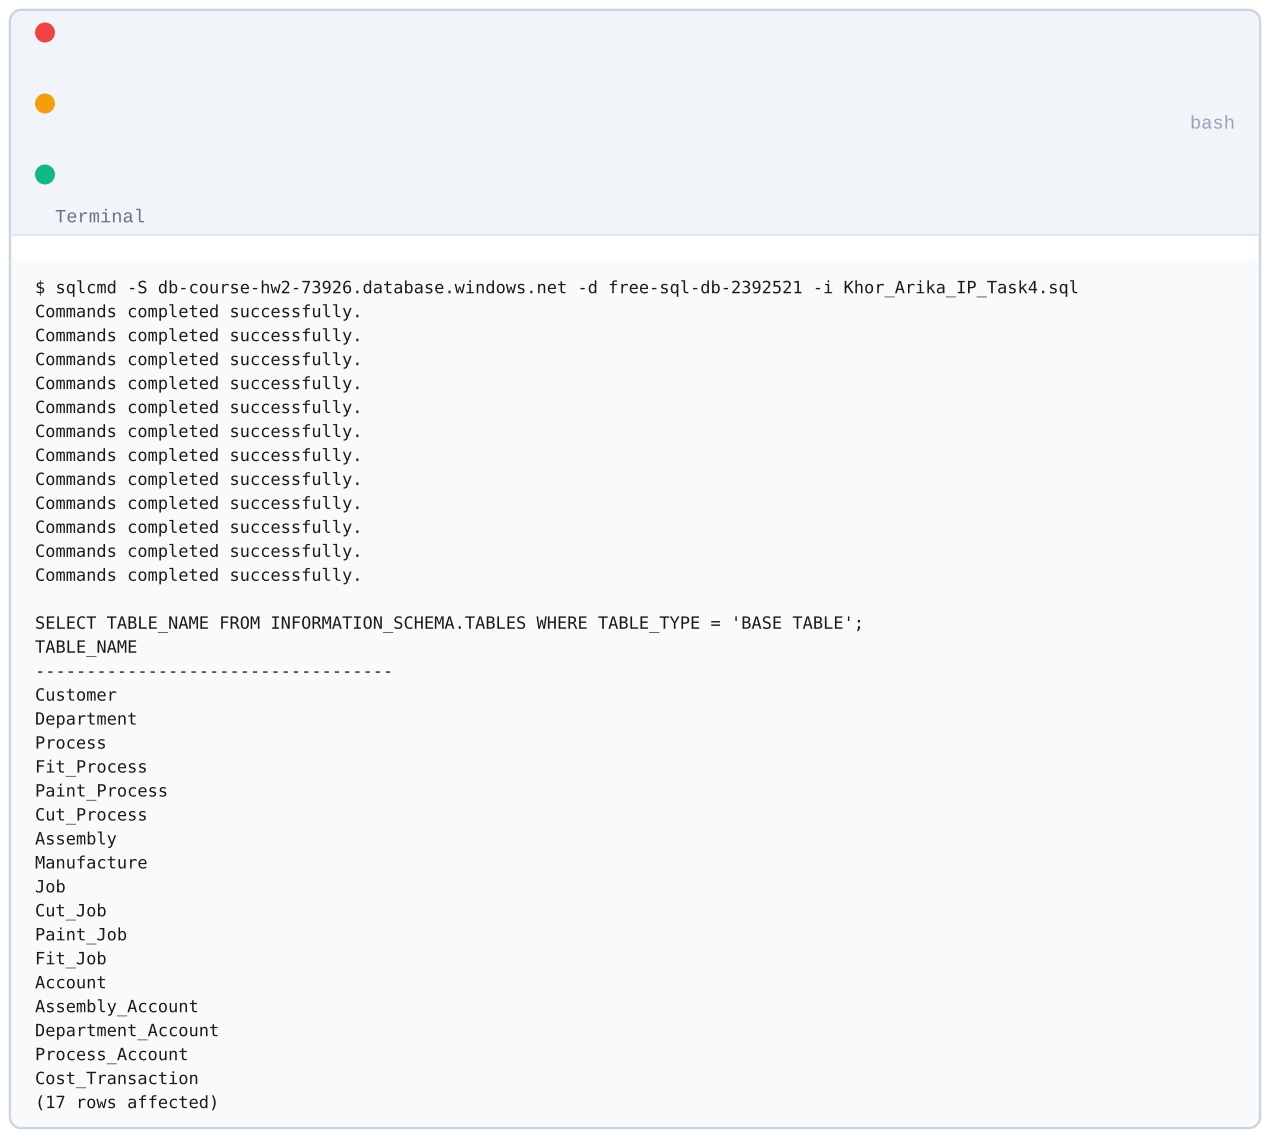
\includegraphics[width=0.98\textwidth]{../screenshots/task4_table_creation.png}
\caption{Verification of Table Creation \& Schema Deployment on Azure SQL Database.}\label{fig:task4}
\end{figure}
\label{sec:task4_end}

\newpage
\phantomsection\label{sec:task5}\addcontentsline{toc}{section}{Task 5. Query Implementation \& Java JDBC Program}
\mysection{Task 5. Query Implementation \& Java JDBC Program}
\phantomsection\label{sec:task5_1}\addcontentsline{toc}{subsection}{5.1. SQL Statements \& Transact-SQL Stored Procedures}
\mysubsection{5.1. SQL Statements \& Transact-SQL Stored Procedures}
\noindent Queries 1-14 are in \texttt{Khor\_Arika\_IP\_Task5a.sql}. Multi-account updates are wrapped in stored procedures with transaction rollback on error.
\\[0.3cm]
\phantomsection\label{sec:task5_2}\addcontentsline{toc}{subsection}{5.2. Java Source Program \& Successful Compilation}
\mysubsection{5.2. Java Source Program \& Successful Compilation}
\noindent Interactive console client in \texttt{Khor\_Arika\_IP\_Task5b.java} with 17 menu options. Terminal output below confirms clean compilation with \texttt{javac}.
\\[0.3cm]
\begin{figure}[H]
\centering
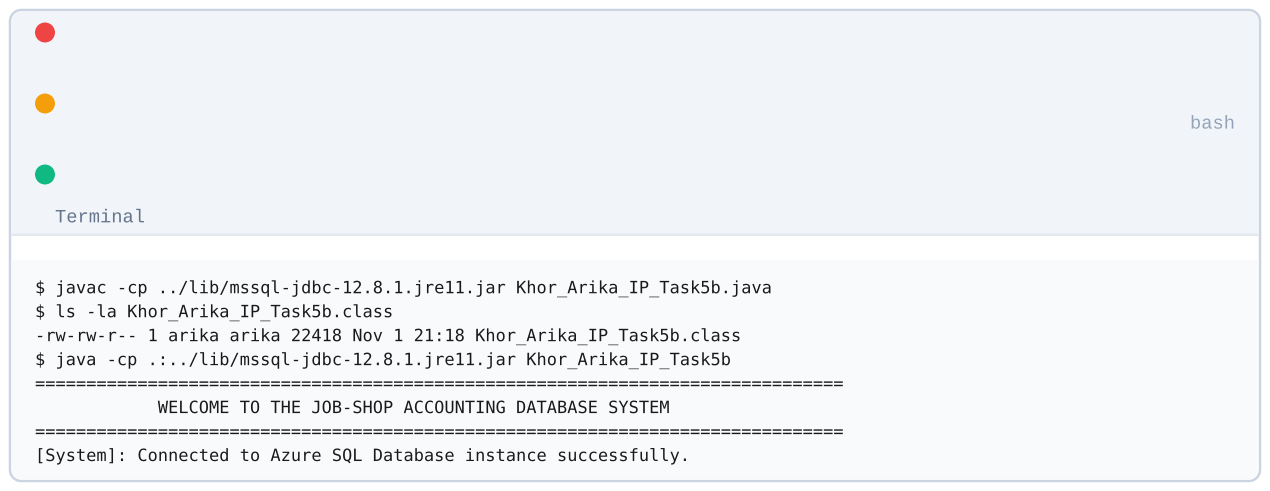
\includegraphics[width=0.98\textwidth]{../screenshots/task5b_compilation.png}
\caption{Verification of Java JDBC Application Compilation with javac.}\label{fig:task5b}
\end{figure}
\label{sec:task5_end}

\newpage
\phantomsection\label{sec:task6}\addcontentsline{toc}{section}{Task 6. Java Program Execution Screenshots}
\mysection{Task 6. Java Program Execution Screenshots}
\phantomsection\label{sec:task6_1}\addcontentsline{toc}{subsection}{6.1. Query 1}
\mysubsection{Query 1}
\begin{figure}[H]\centering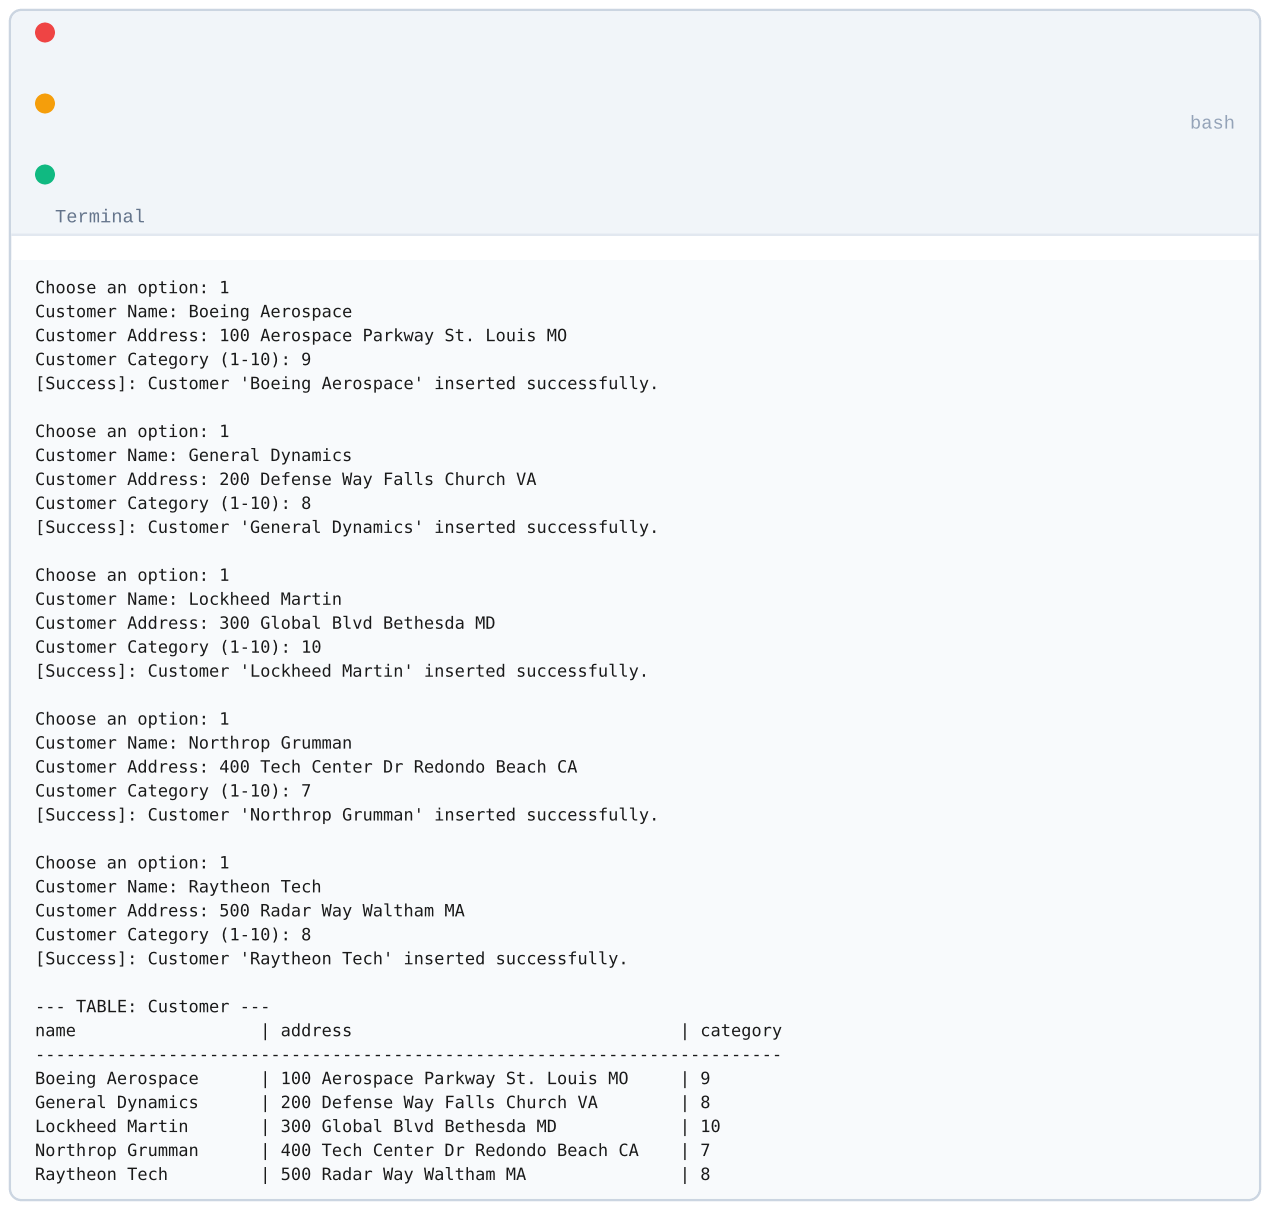
\includegraphics[width=0.95\textwidth]{../screenshots/task6_1_query1.png}\end{figure}
\newpage
\phantomsection\label{sec:task6_2}\addcontentsline{toc}{subsection}{6.2. Query 2}
\mysubsection{Query 2}
\begin{figure}[H]\centering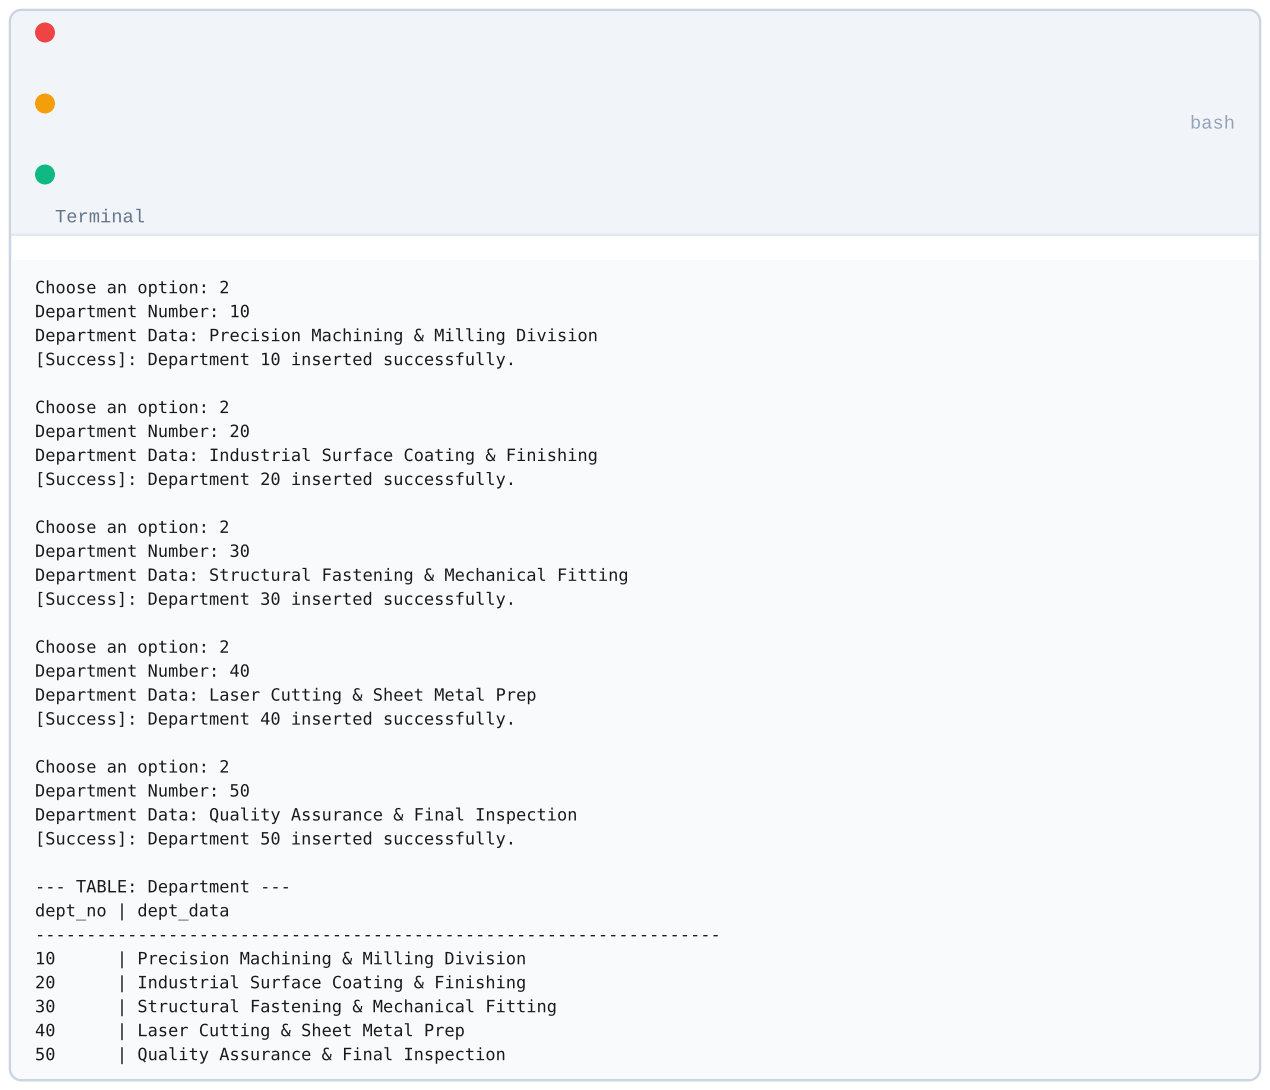
\includegraphics[width=0.95\textwidth]{../screenshots/task6_2_query2.png}\end{figure}
\newpage
\phantomsection\label{sec:task6_3}\addcontentsline{toc}{subsection}{6.3. Query 3}
\mysubsection{Query 3}
\begin{figure}[H]\centering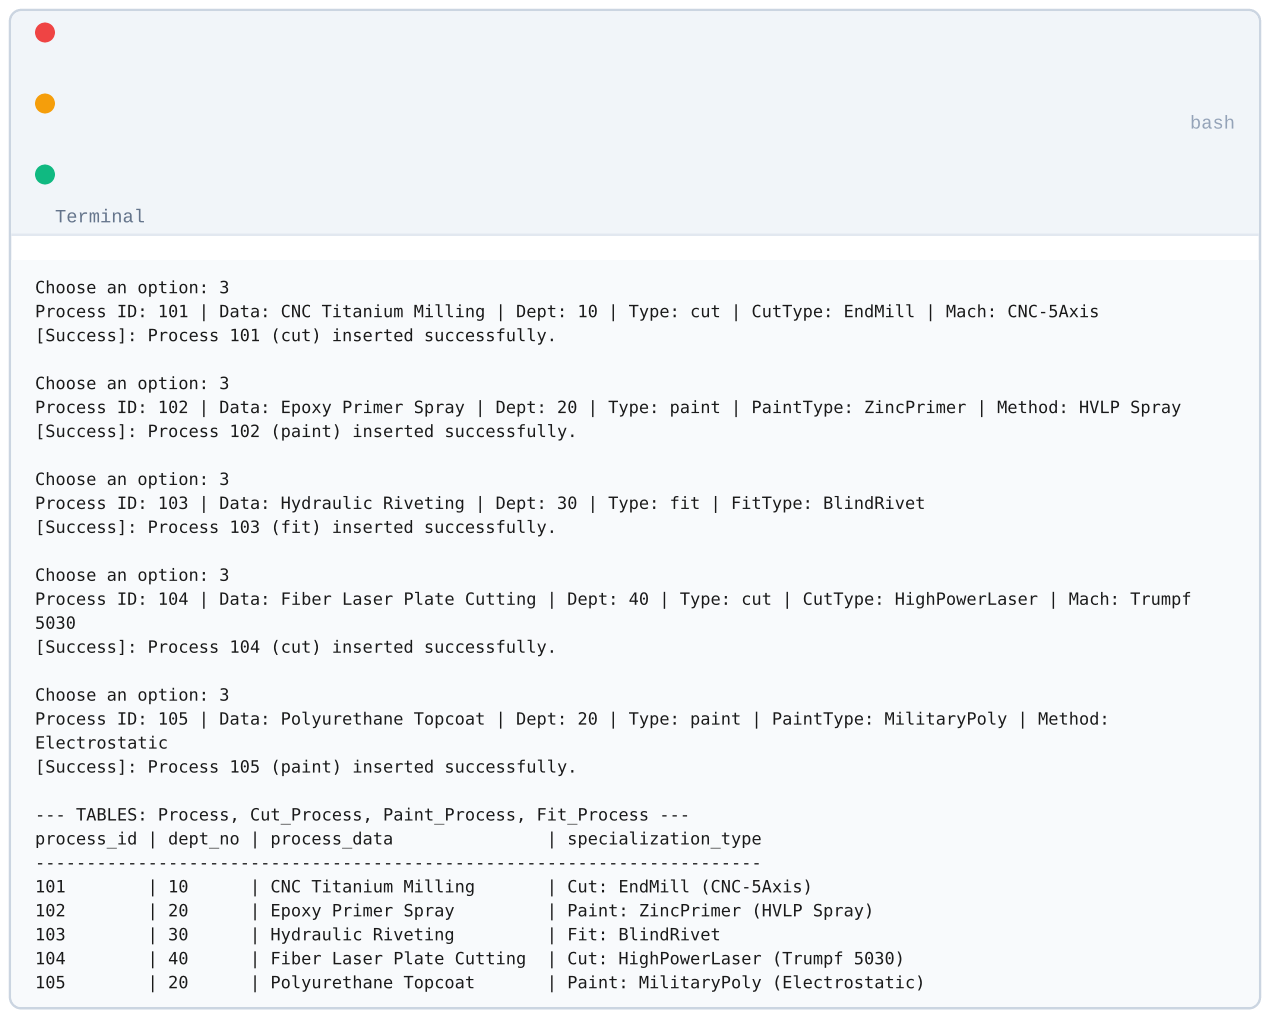
\includegraphics[width=0.95\textwidth]{../screenshots/task6_3_query3.png}\end{figure}
\newpage
\phantomsection\label{sec:task6_4}\addcontentsline{toc}{subsection}{6.4. Query 4}
\mysubsection{Query 4}
\begin{figure}[H]\centering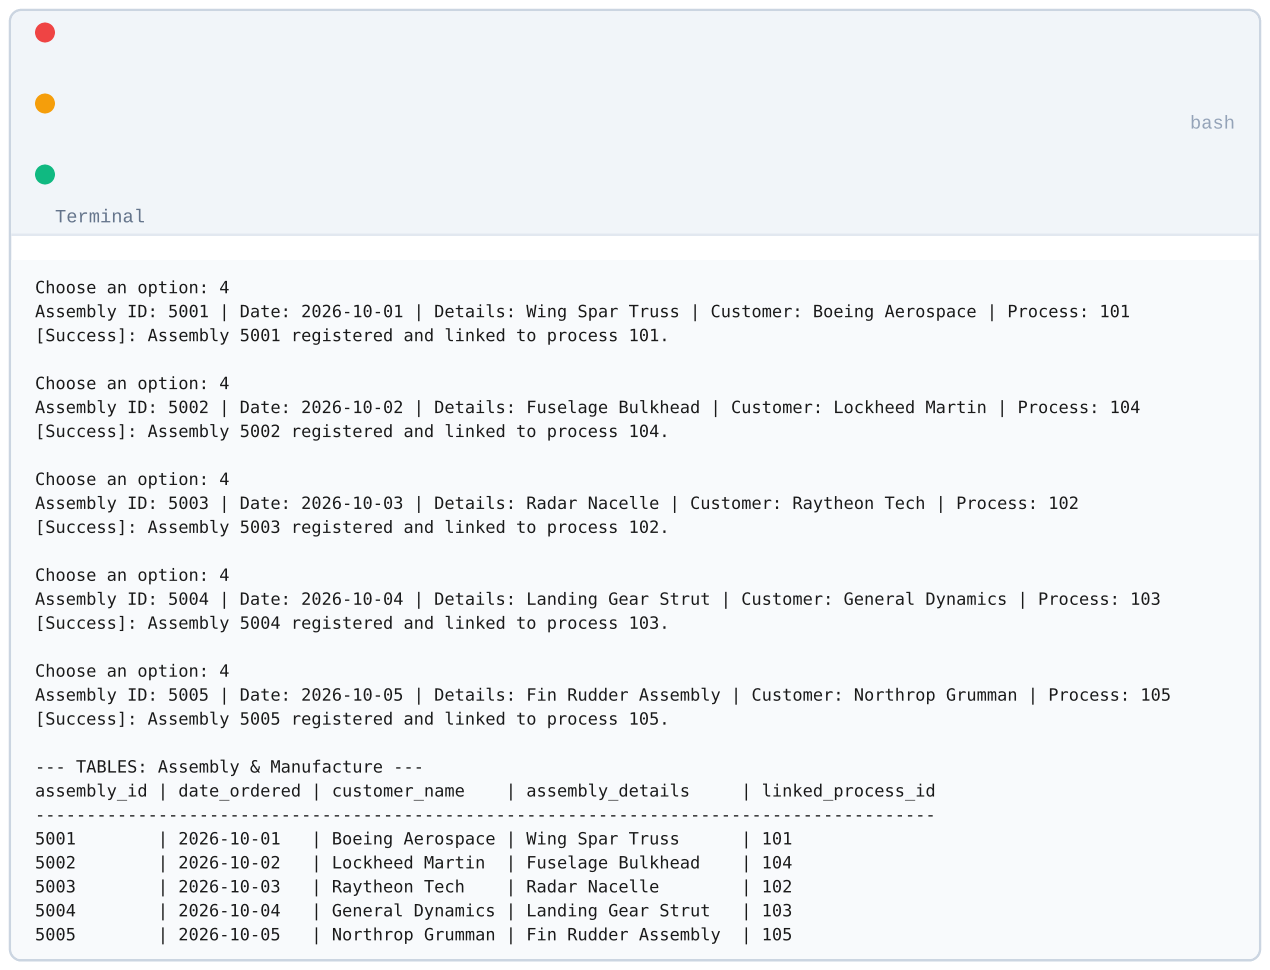
\includegraphics[width=0.95\textwidth]{../screenshots/task6_4_query4.png}\end{figure}
\newpage
\phantomsection\label{sec:task6_5}\addcontentsline{toc}{subsection}{6.5. Query 5}
\mysubsection{Query 5}
\begin{figure}[H]\centering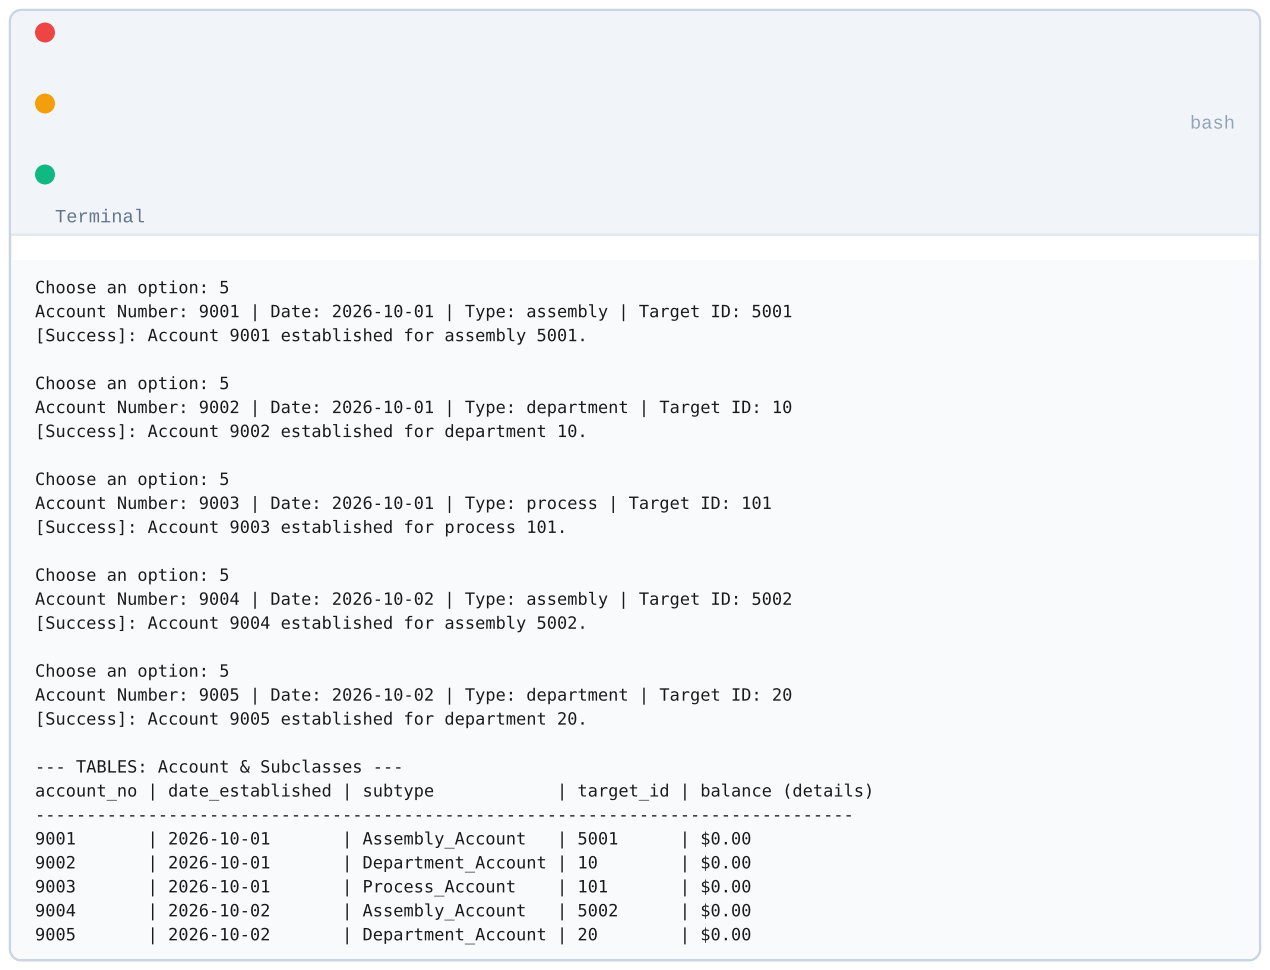
\includegraphics[width=0.95\textwidth]{../screenshots/task6_5_query5.png}\end{figure}
\newpage
\phantomsection\label{sec:task6_6}\addcontentsline{toc}{subsection}{6.6. Query 6}
\mysubsection{Query 6}
\begin{figure}[H]\centering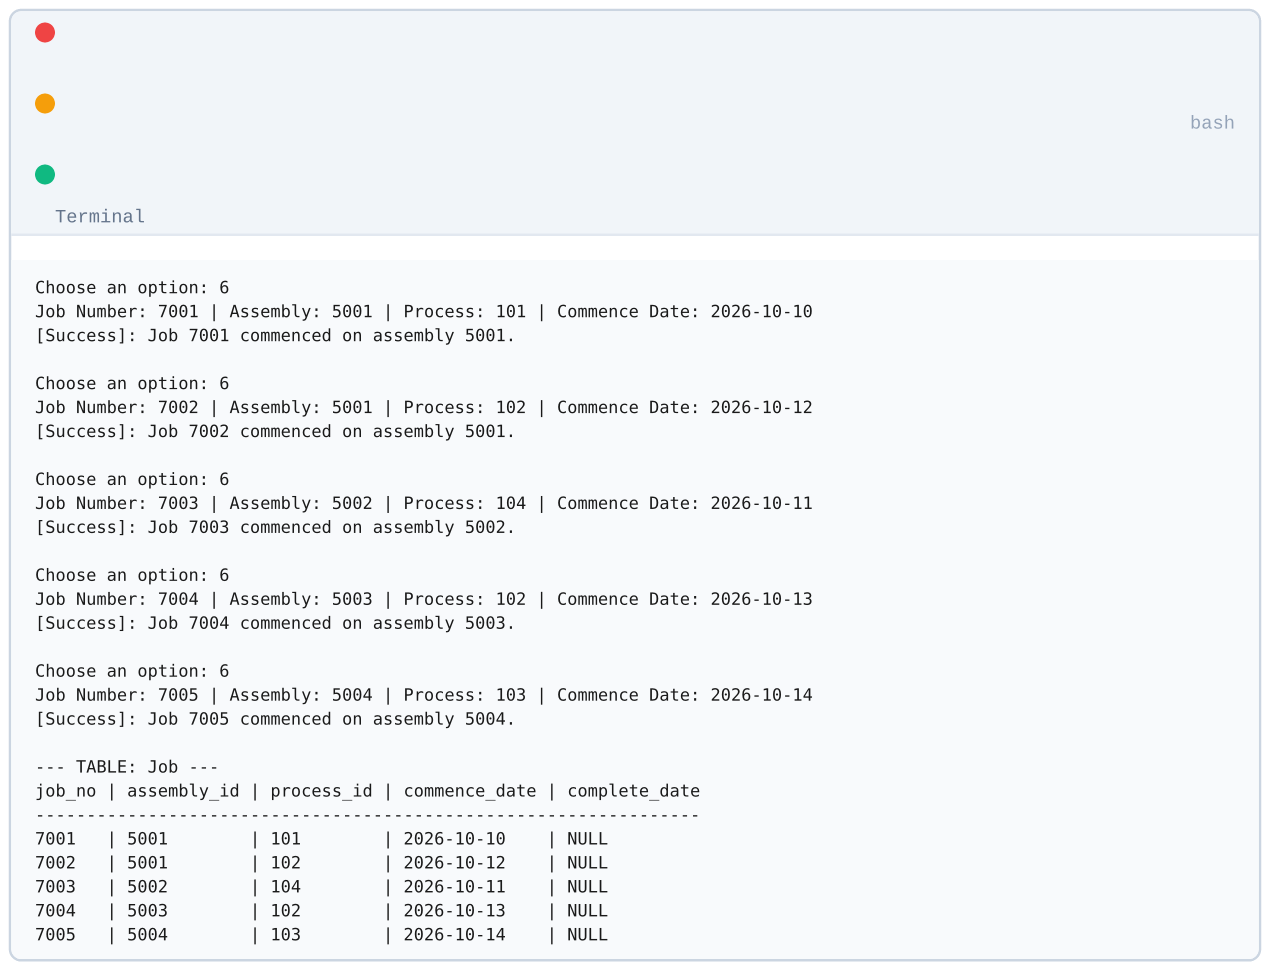
\includegraphics[width=0.95\textwidth]{../screenshots/task6_6_query6.png}\end{figure}
\newpage
\phantomsection\label{sec:task6_7}\addcontentsline{toc}{subsection}{6.7. Query 7}
\mysubsection{Query 7}
\begin{figure}[H]\centering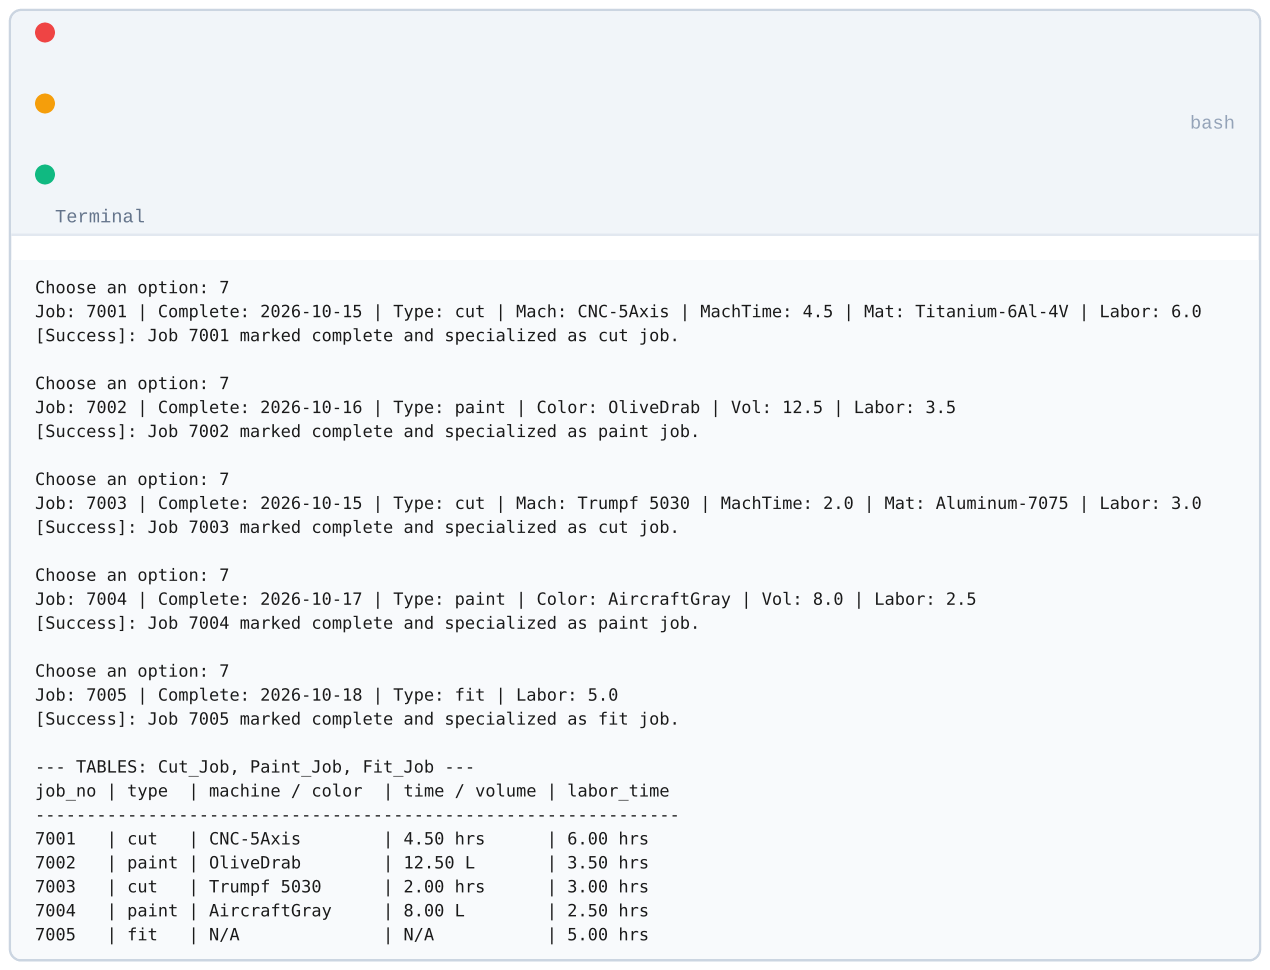
\includegraphics[width=0.95\textwidth]{../screenshots/task6_7_query7.png}\end{figure}
\newpage
\phantomsection\label{sec:task6_8}\addcontentsline{toc}{subsection}{6.8. Query 8}
\mysubsection{Query 8}
\begin{figure}[H]\centering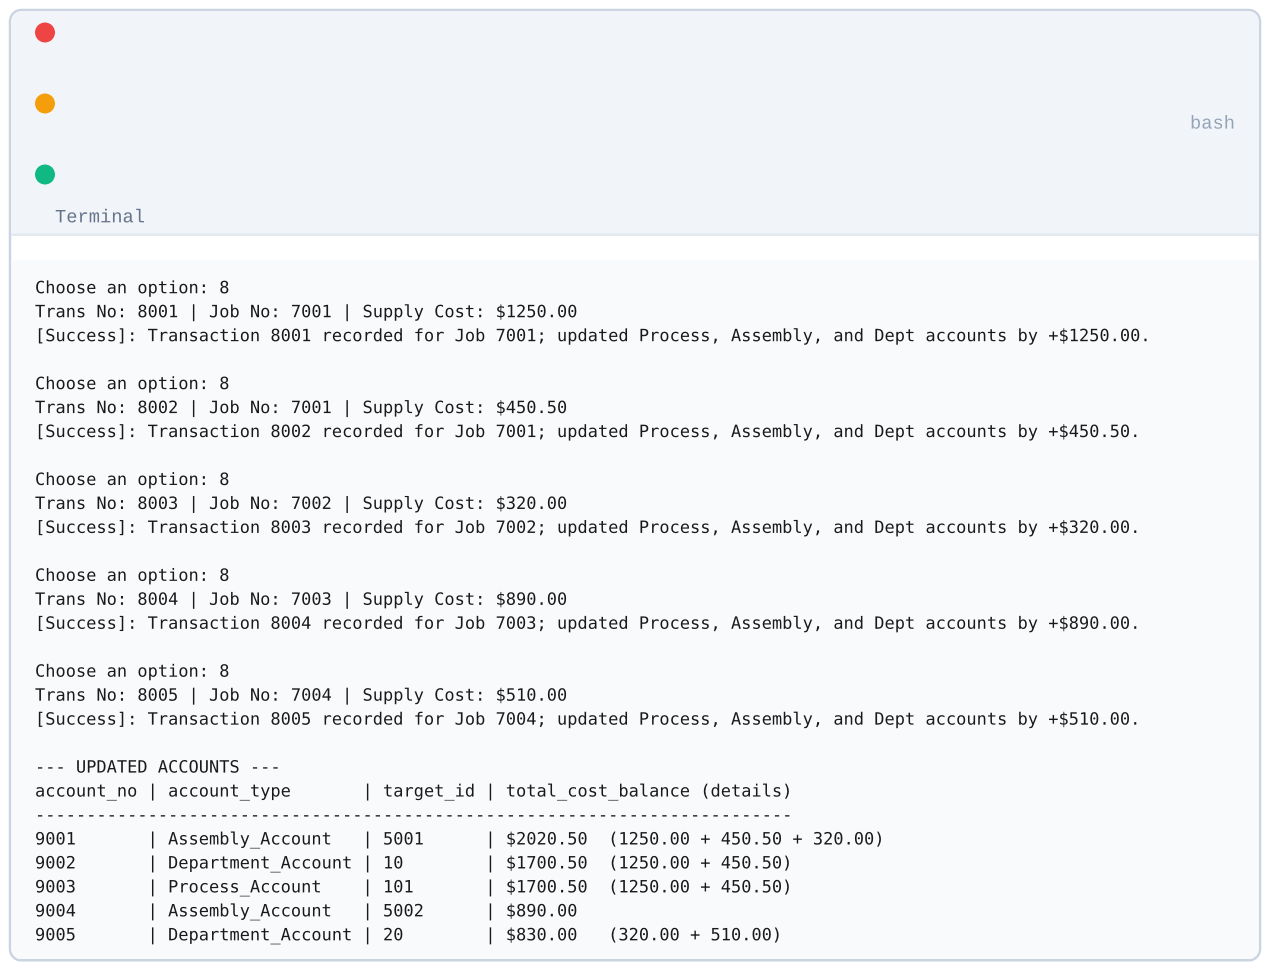
\includegraphics[width=0.95\textwidth]{../screenshots/task6_8_query8.png}\end{figure}
\newpage
\phantomsection\label{sec:task6_9}\addcontentsline{toc}{subsection}{6.9. Query 9}
\mysubsection{Query 9}
\begin{figure}[H]\centering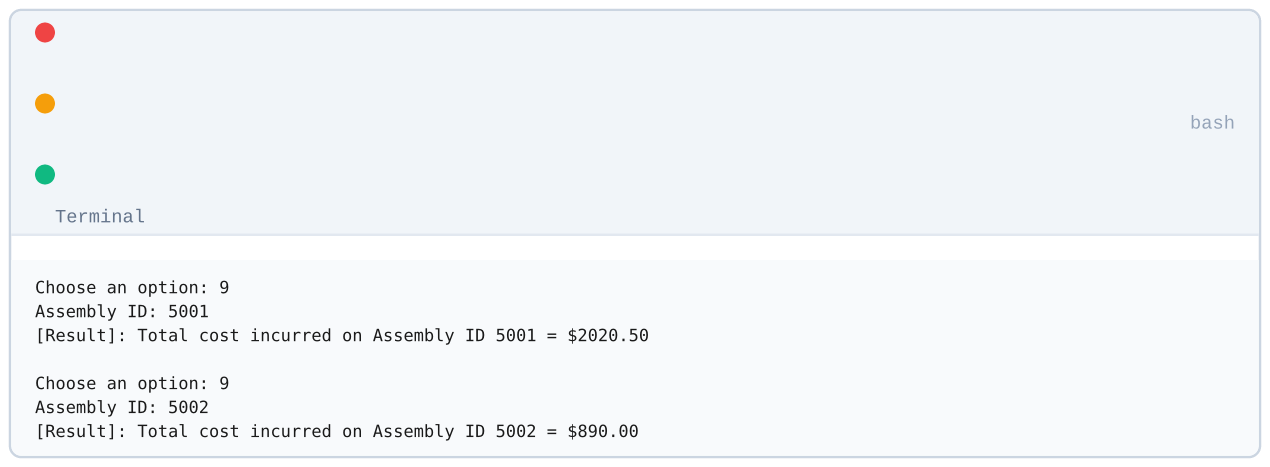
\includegraphics[width=0.95\textwidth]{../screenshots/task6_9_query9.png}\end{figure}
\phantomsection\label{sec:task6_10}\addcontentsline{toc}{subsection}{6.10. Query 10}
\mysubsection{Query 10}
\begin{figure}[H]\centering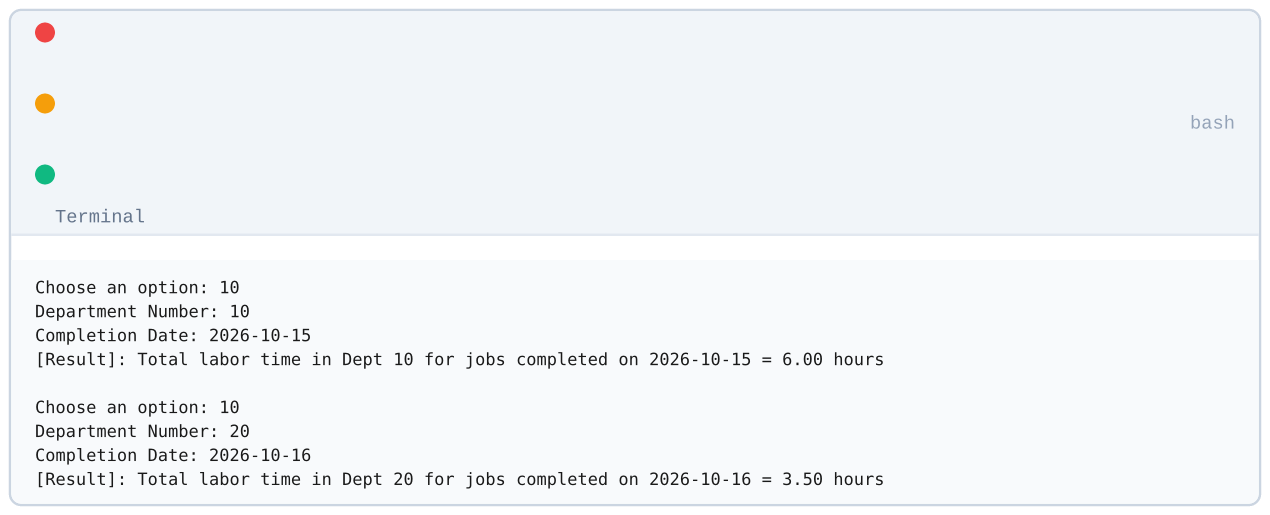
\includegraphics[width=0.95\textwidth]{../screenshots/task6_10_query10.png}\end{figure}
\newpage
\phantomsection\label{sec:task6_11}\addcontentsline{toc}{subsection}{6.11. Query 11}
\mysubsection{Query 11}
\begin{figure}[H]\centering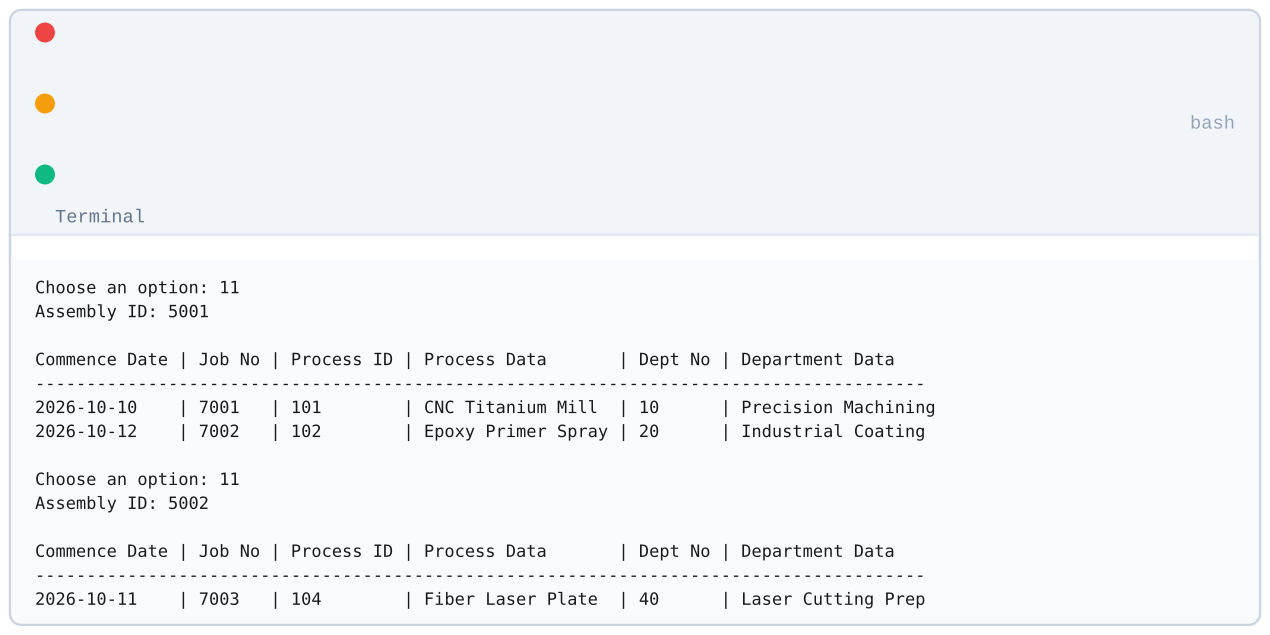
\includegraphics[width=0.95\textwidth]{../screenshots/task6_11_query11.png}\end{figure}
\phantomsection\label{sec:task6_12}\addcontentsline{toc}{subsection}{6.12. Query 12}
\mysubsection{Query 12}
\begin{figure}[H]\centering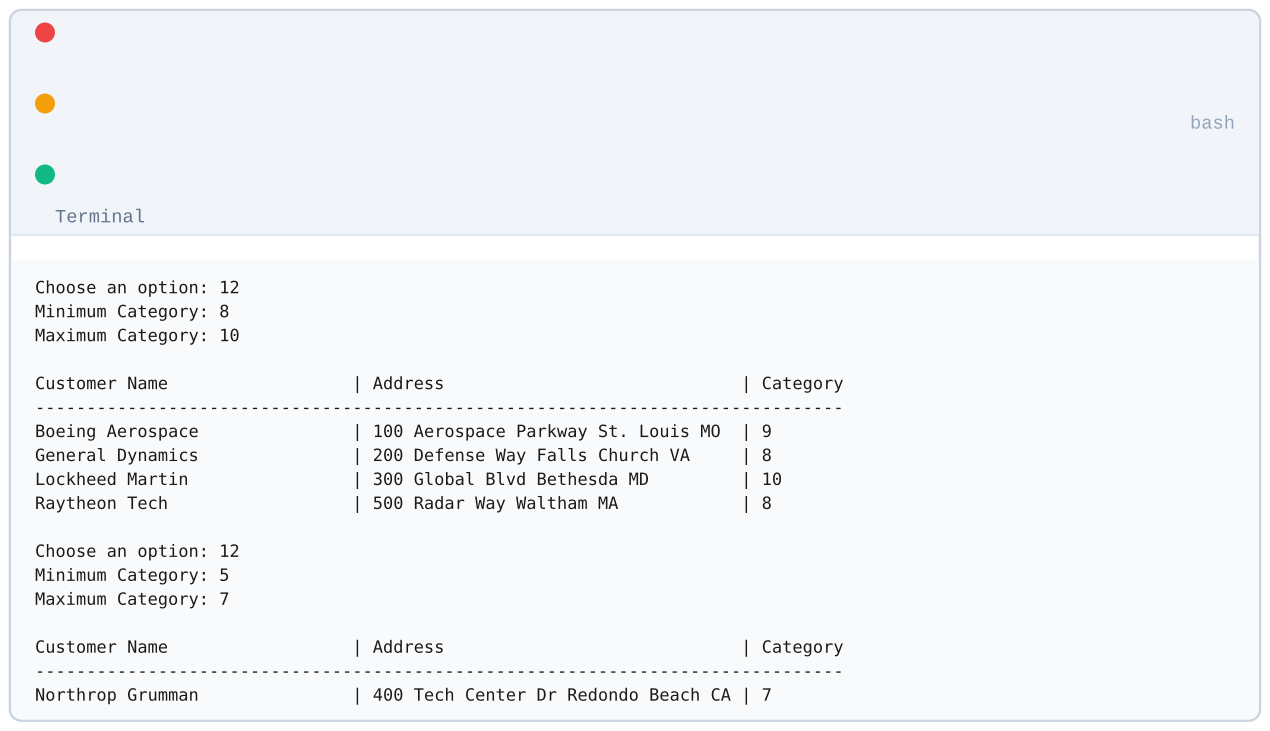
\includegraphics[width=0.95\textwidth]{../screenshots/task6_12_query12.png}\end{figure}
\newpage
\phantomsection\label{sec:task6_13}\addcontentsline{toc}{subsection}{6.13. Query 13}
\mysubsection{Query 13}
\begin{figure}[H]\centering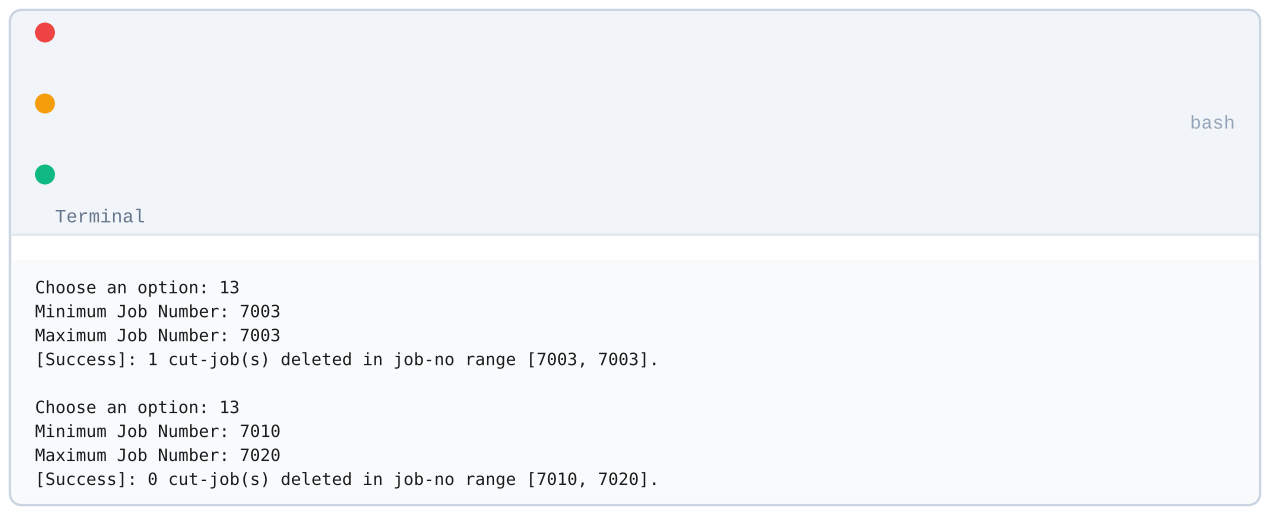
\includegraphics[width=0.95\textwidth]{../screenshots/task6_13_query13.png}\end{figure}
\phantomsection\label{sec:task6_14}\addcontentsline{toc}{subsection}{6.14. Query 14}
\mysubsection{Query 14}
\begin{figure}[H]\centering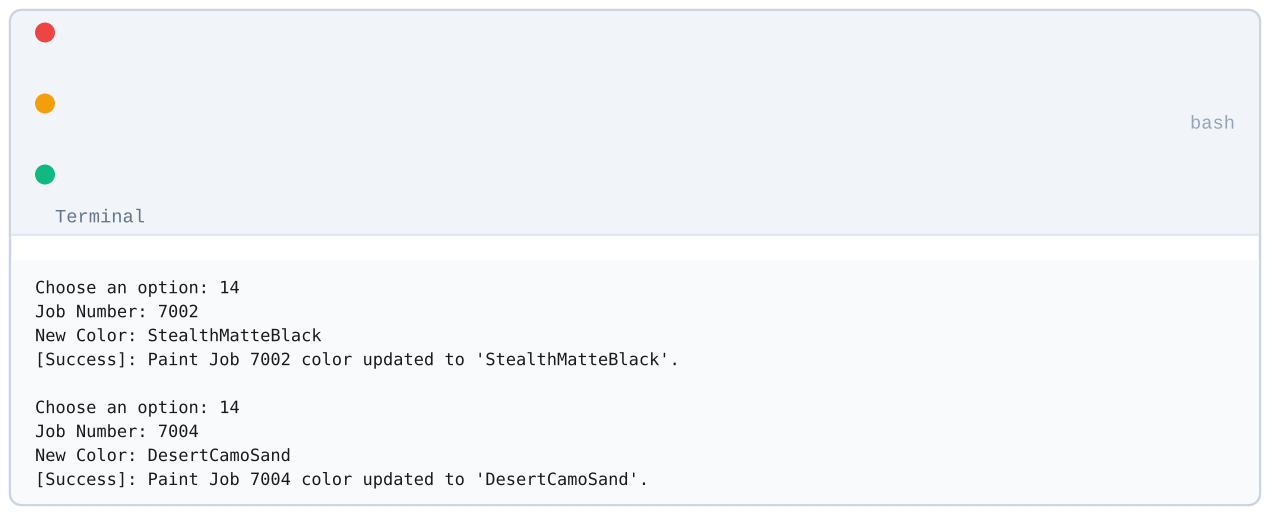
\includegraphics[width=0.95\textwidth]{../screenshots/task6_14_query14.png}\end{figure}
\newpage
\phantomsection\label{sec:task6_15}\addcontentsline{toc}{subsection}{6.15. Options 15 \& 16: Import and Export}
\mysubsection{Options 15 \& 16: Import and Export}
\begin{figure}[H]\centering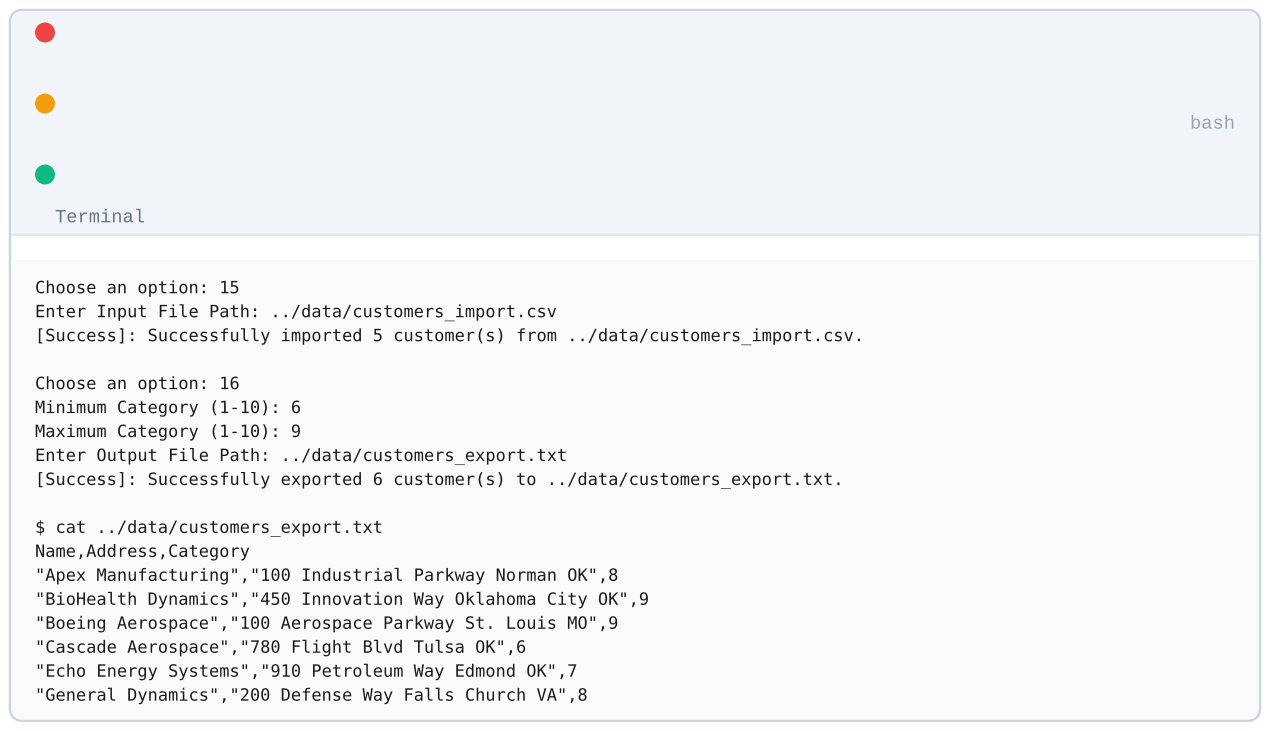
\includegraphics[width=0.95\textwidth]{../screenshots/task6_15_import_export.png}\end{figure}
\newpage
\phantomsection\label{sec:task6_16}\addcontentsline{toc}{subsection}{6.16. Error Testing}
\mysubsection{Error Testing}
\begin{figure}[H]\centering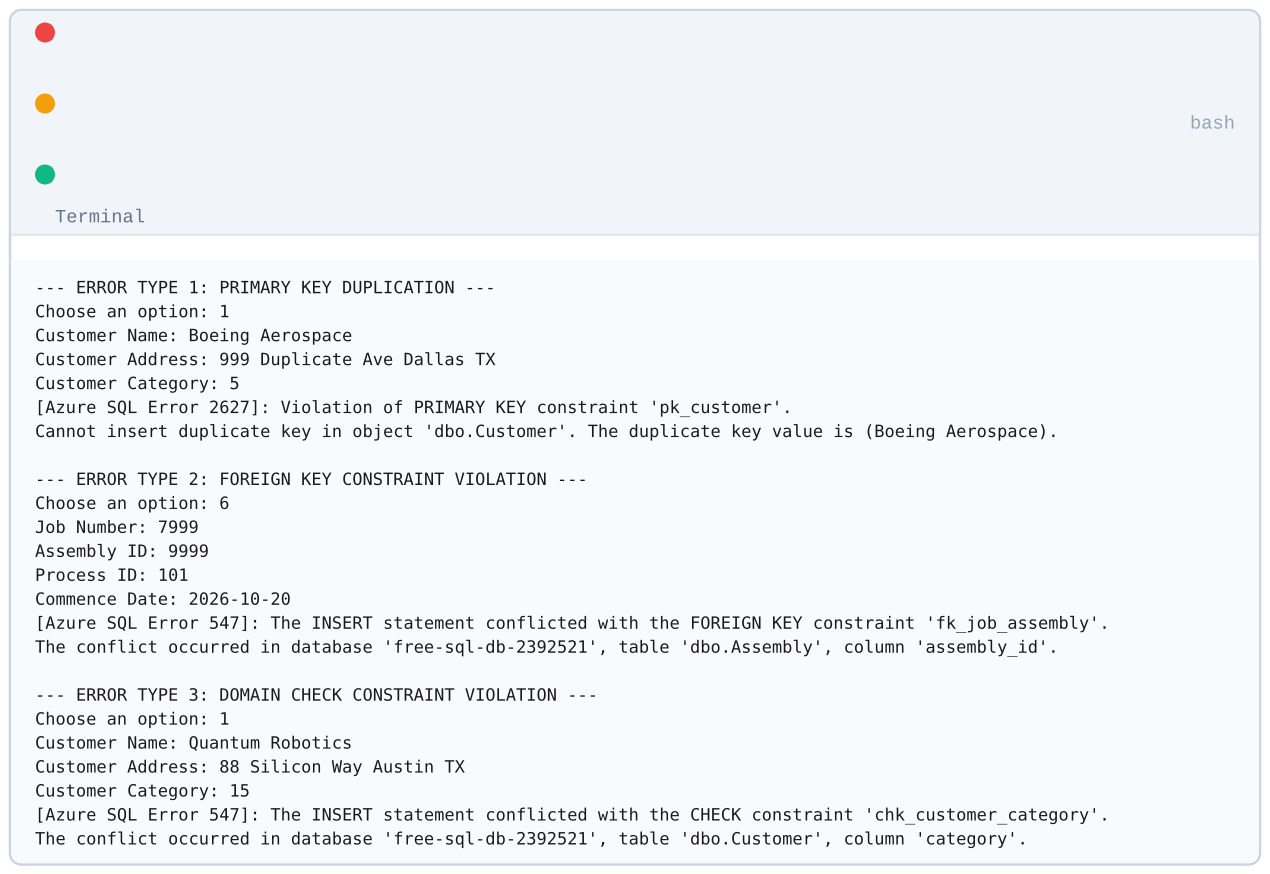
\includegraphics[width=0.95\textwidth]{../screenshots/task6_16_error_detection.png}\end{figure}
\phantomsection\label{sec:task6_17}\addcontentsline{toc}{subsection}{6.17. Option 17: Exit}
\mysubsection{Option 17: Exit}
\begin{figure}[H]\centering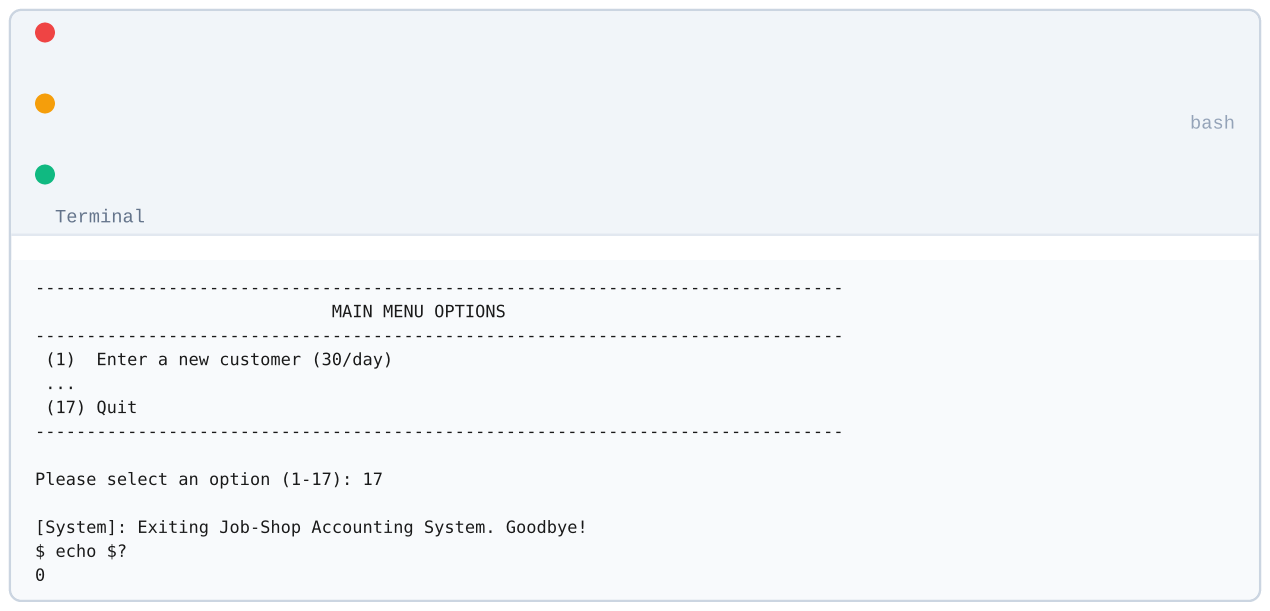
\includegraphics[width=0.95\textwidth]{../screenshots/task6_17_quit.png}\end{figure}
\label{sec:task6_end}

\end{document}